\documentclass[conference]{IEEEtran}
\usepackage{graphicx}
\usepackage{amsmath}
\usepackage{cite}
\usepackage{booktabs}
\usepackage{url}

\begin{document}

\title{A Multilayer Perceptron Trained by Particle Swarm Optimisation}

\author{
\IEEEauthorblockN{[Your name(s) here]}
\IEEEauthorblockA{Biologically Inspired Computation\\{}
[Institution name]\\{}
[Date]}
}

\maketitle

\begin{abstract}
This paper presents a generic Multilayer Perceptron (MLP), implemented from
scratch using NumPy, whose weights and biases are optimised by Particle
Swarm Optimisation (PSO) rather than gradient descent. The MLP and PSO
components are implemented independently and connected through an adapter,
so that the optimisation algorithm has no knowledge of neural-network
internals. On a placeholder dataset (Iris), the best configuration achieved
a training loss of 0.087 and a test accuracy of 0.967. We additionally
compare random and nearest-neighbour informant-selection strategies for PSO,
and the effect of swarm size on convergence.
\end{abstract}

\begin{IEEEkeywords}
particle swarm optimisation, multilayer perceptron, neuroevolution,
informant selection, swarm intelligence
\end{IEEEkeywords}

\section{Introduction}
Gradient descent is the conventional way to train a neural network, but it
is not the only option: any algorithm capable of minimising a scalar
objective over a continuous parameter space can, in principle, train one.
This work treats a Multilayer Perceptron's entire set of weights and biases
as a single point in a high-dimensional search space, and uses Particle
Swarm Optimisation (PSO) -- a population-based, biologically inspired
search algorithm modelled on the collective movement of bird flocks and
fish schools -- to search that space directly for a parameter vector that
minimises training loss.

[Add: one or two sentences on the dataset/problem you chose, and why. State
the task type -- binary or multiclass classification -- explicitly.]

\section{Design}

\subsection{Component independence}
The implementation is split into two independent components connected by a
single adapter, so that the optimisation algorithm has no knowledge of
neural networks and the network has no knowledge of how its parameters are
chosen (Table~\ref{tab:components}).

\begin{table}[h]
\caption{System components and responsibilities}
\label{tab:components}
\centering
\begin{tabular}{p{0.18\linewidth}p{0.52\linewidth}p{0.2\linewidth}}
\toprule
\textbf{Component} & \textbf{Responsibility} & \textbf{Key classes} \\
\midrule
MLP & Represents the network: stores weights/biases, performs a forward
pass, computes a loss. & \texttt{Layer}, \texttt{Network},
\texttt{MLPBuilder} \\
PSO & Generic population-based search minimising a scalar fitness
function. & \texttt{Particle}, \texttt{Population},
\texttt{InformantSelectionStrategy} \\
Adapter & Connects the two: evaluates an MLP's training loss for a
candidate parameter vector. & \texttt{MLPFitnessAdapter} \\
\bottomrule
\end{tabular}
\end{table}

\subsection{Design patterns}
Three design patterns structure the implementation (Table~\ref{tab:patterns}).

\begin{table}[h]
\caption{Design patterns and the problem each solves}
\label{tab:patterns}
\centering
\begin{tabular}{p{0.16\linewidth}p{0.56\linewidth}p{0.18\linewidth}}
\toprule
\textbf{Pattern} & \textbf{Problem solved} & \textbf{Where} \\
\midrule
Builder & Constructs a complete network from a small hyperparameter
configuration, without manual layer creation. & \texttt{MLPBuilder.build()} \\
Strategy & Makes informant selection swappable (random vs.\
nearest-neighbour) without changing \texttt{Particle} or \texttt{Population}.
& \texttt{InformantSelectionStrategy} \\
Adapter & Lets PSO call a single \texttt{evaluate(position)} method without
knowledge of layers, weights, or loss functions. & \texttt{MLPFitnessAdapter} \\
\bottomrule
\end{tabular}
\end{table}

[Add 1--2 sentences per pattern justifying the choice -- e.g. why Strategy
specifically, rather than a conditional branch, matters for extensibility.]

\subsection{Parameter vector representation}
PSO searches over real-valued vectors, so the network's weights and biases
across every layer are flattened into a single vector of length $D$
(weights then biases, per layer, in order), and can be reconstructed from
any vector of that length. This is what makes a particle's position
equivalent to a candidate set of network parameters:
\begin{equation}
D = \sum_{l=1}^{L} \left( n_{l-1} \cdot n_l + n_l \right)
\label{eq:dimension}
\end{equation}
where $n_{l-1}$ and $n_l$ are the sizes of the preceding and current layer.
For the architecture used in this report, $D = $ [fill in from
\texttt{network.count\_parameters()}].

\subsection{PSO update equations}
Each particle's velocity combines inertia, a pull toward its own personal
best, and a pull toward the best position among its informants:
\begin{equation}
v_i(t\!+\!1) = \alpha v_i(t) + \beta r_1 (p_i^{best} - x_i(t)) +
\delta r_2 (p_i^{I} - x_i(t))
\label{eq:velocity}
\end{equation}
\begin{equation}
x_i(t+1) = x_i(t) + \varepsilon \, v_i(t+1)
\label{eq:position}
\end{equation}
where $\alpha$ is the inertia weight, $\beta$ the cognitive coefficient,
$\delta$ the social coefficient, $\varepsilon$ the step size, and $r_1,
r_2$ are random values drawn fresh each iteration. Informants are
reassigned every iteration using the configured
\texttt{InformantSelectionStrategy}.

\section{Methodology}

\subsection{Dataset}
[Describe: source, number of samples, number of features, number of
classes, class balance, train/test split ratio and method (e.g.\ stratified
80/20), and any preprocessing -- note that any scaler must be fit on
training data only.]

\subsection{Network architecture}
\begin{table}[h]
\caption{Network hyperparameters used}
\label{tab:network}
\centering
\begin{tabular}{ll}
\toprule
\textbf{Hyperparameter} & \textbf{Value used} \\
\midrule
Hidden layers & [e.g.\ 8, 5] \\
Hidden activations & [e.g.\ tanh, sigmoid] \\
Task type & [binary / multiclass classification] \\
Output activation / loss & [Sigmoid+BCE or Softmax+CCE] \\
\bottomrule
\end{tabular}
\end{table}

\subsection{PSO configuration}
\begin{table}[h]
\caption{PSO hyperparameters tested}
\label{tab:pso}
\centering
\begin{tabular}{ll}
\toprule
\textbf{Hyperparameter} & \textbf{Value(s) tested} \\
\midrule
Particles ($N$) & [e.g.\ 10, 30, 60] \\
Informants ($k$) & [value, $1 \le k \le N-1$] \\
Iterations & [e.g.\ 150] \\
Inertia weight ($\alpha$) & [value(s)] \\
Cognitive coefficient ($\beta$) & [value(s)] \\
Social coefficient ($\delta$) & [value(s)] \\
Informant strategy & Random vs.\ Nearest-Neighbour \\
\bottomrule
\end{tabular}
\end{table}

\subsection{Evaluation protocol}
The \texttt{MLPFitnessAdapter} evaluates every candidate solution using
only the training set; the test set is never seen during optimisation.
After PSO returns its best parameter vector, that vector is installed into
the network once, and accuracy, precision, recall and F1-score
(macro-averaged) are computed on the held-out test set only.

\section{Results}

\subsection{Training and test performance}
\begin{table}[h]
\caption{Example results on a placeholder dataset (Iris)}
\label{tab:results}
\centering
\begin{tabular}{lc}
\toprule
\textbf{Metric} & \textbf{Value} \\
\midrule
Best training loss & 0.087 \\
Test accuracy & 0.967 \\
Test precision (macro) & 0.970 \\
Test recall (macro) & 0.967 \\
Test F1-score (macro) & 0.967 \\
\bottomrule
\end{tabular}
\end{table}
\noindent \textit{Replace with your team's actual dataset results.}

\subsection{PSO convergence}
\begin{figure}[h]
\centering
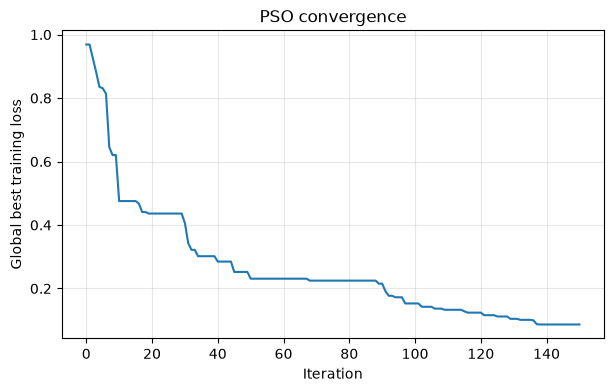
\includegraphics[width=0.95\linewidth]{plot_1.png}
\caption{Global-best training loss versus iteration. [Describe the shape:
how quickly it drops, where it plateaus, and whether it fully converged
within the iteration budget.]}
\label{fig:convergence}
\end{figure}

\subsection{Informant-strategy comparison}
\begin{table}[h]
\caption{Random vs.\ Nearest-Neighbour informant selection}
\label{tab:informants}
\centering
\begin{tabular}{lcc}
\toprule
\textbf{Strategy} & \textbf{Best loss} & \textbf{Test acc.} \\
\midrule
Random & 0.353 & 0.867 \\
Nearest-Neighbour & 0.087 & 0.967 \\
\bottomrule
\end{tabular}
\end{table}

\begin{figure}[h]
\centering
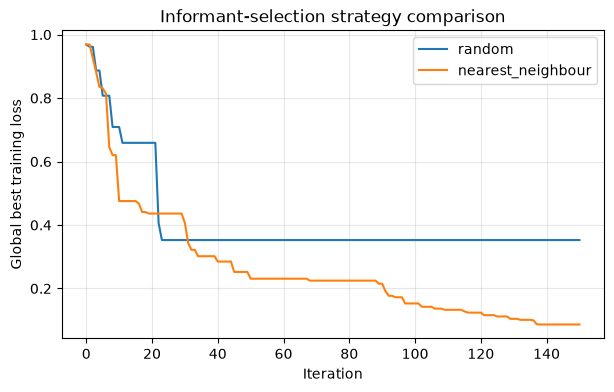
\includegraphics[width=0.95\linewidth]{plot_2.png}
\caption{Convergence under Random vs.\ Nearest-Neighbour informant
selection, same PSO settings otherwise.}
\label{fig:informants}
\end{figure}

[Run this comparison across several random seeds and report mean $\pm$
standard deviation rather than a single run -- PSO is stochastic.]

\subsection{Hyperparameter comparison}
\begin{table}[h]
\caption{Effect of swarm size on best training loss}
\label{tab:swarmsize}
\centering
\begin{tabular}{lc}
\toprule
\textbf{Particles ($N$)} & \textbf{Best training loss} \\
\midrule
10 & 0.168 \\
30 & 0.087 \\
60 & 0.086 \\
\bottomrule
\end{tabular}
\end{table}

\begin{figure}[h]
\centering
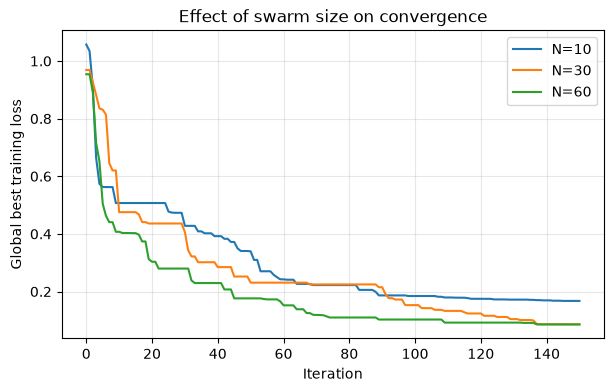
\includegraphics[width=0.95\linewidth]{plot_3.png}
\caption{Effect of swarm size on convergence. [Add at least one more
hyperparameter axis, e.g.\ inertia weight or hidden-layer size.]}
\label{fig:swarmsize}
\end{figure}

\section{Discussion}
[Explain WHY the results look the way they do, referring back to the
mechanics in Section~II -- e.g.\ why nearest-neighbour informants might
converge faster/more reliably than random ones; why larger swarms show
diminishing returns; any runs that got stuck or diverged, and what
hyperparameter choice caused it.]

\subsection{Limitations}
[e.g.\ results are from single runs per configuration; PSO's stochasticity
means conclusions should be validated across multiple seeds; dataset
size/complexity limits generalisability of conclusions about
hyperparameters.]

\section{Conclusion}
[Summarise what was built, what worked best, and one or two concrete next
steps you would try with more time -- e.g.\ multi-seed averaging,
hybridising PSO with local search, testing deeper architectures.]

\begin{thebibliography}{1}

\bibitem{kennedy1995}
J.~Kennedy and R.~Eberhart, ``Particle swarm optimization,'' in
\textit{Proc. ICNN'95 -- Int. Conf. Neural Networks}, vol.~4, 1995,
pp.~1942--1948.

\bibitem{dataset}
[Dataset citation -- e.g.\ the UCI/sklearn source of your chosen dataset.]

\bibitem{repo}
[Your GitHub repository link, e.g.\ \url{https://github.com/mr1pro/bio-inspired-pso-notebook}.]

\end{thebibliography}

\end{document}
